

\chapter{Classes and objects}
\label{clobjects}

At this point you know how to use
functions to organize code and
built-in types to organize data.  The next step is to learn
``object-oriented programming'', which uses programmer-defined types
to organize both code and data.  Object-oriented programming is
a big topic; it will take a few chapters to get there.
\index{object-oriented programming}

Code examples from this chapter are available from
\url{http://thinkpython2.com/code/Point1.py}; solutions
to the exercises are available from
\url{http://thinkpython2.com/code/Point1_soln.py}.


\section{Programmer-defined types}
\label{point}
\index{programmer-defined type}  \index{type!programmer-defined}

We have used many of Python's built-in types; now we are going
to define a new type.  As an example, we will create a type
called {\tt Point} that represents a point in two-dimensional
space.
\index{point, mathematical}

In mathematical notation, points are often written in
parentheses with a comma separating the coordinates. For example,
$(0,0)$ represents the origin, and $(x,y)$ represents the
point $x$ units to the right and $y$ units up from the origin.

There are several ways we might represent points in Python:

\begin{itemize}

\item We could store the coordinates separately in two
variables, {\tt x} and {\tt y}.

\item We could store the coordinates as elements in a list
or tuple.

\item We could create a new type to represent points as
objects.

\end{itemize}
\index{representation}

Creating a new type
is more complicated than the other options, but
it has advantages that will be apparent soon.

A programmer-defined type is also called a {\bf class}.
A class definition looks like this:
\index{class}  \index{object!class}
\index{class definition}  \index{definition!class}

\begin{verbatim}
class Point:
    """Represents a point in 2-D space."""
\end{verbatim}
%
The header indicates that the new class is called {\tt Point}.
The body is a docstring that explains what the class is for.
You can define variables and methods inside a class definition,
but we will get back to that later.
\index{Point class}
\index{class!Point}
\index{docstring}

Defining a class named {\tt Point} creates a {\bf class object}.

\begin{verbatim}
>>> Point
<class '__main__.Point'>
\end{verbatim}
%
Because {\tt Point} is defined at the top level, its ``full
name'' is \verb"__main__.Point".
\index{object!class}
\index{class object}

The class object is like a factory for creating objects.  To create a
Point, you call {\tt Point} as if it were a function.

\begin{verbatim}
>>> blank = Point()
>>> blank
<__main__.Point object at 0xb7e9d3ac>
\end{verbatim}
%
The return value is a reference to a Point object, which we
assign to {\tt blank}.

Creating a new object is called
{\bf instantiation}, and the object is an {\bf instance} of
the class.
\index{instance}
\index{instantiation}

When you print an instance, Python tells you what class it
belongs to and where it is stored in memory (the prefix
{\tt 0x} means that the following number is in hexadecimal).
\index{hexadecimal}

Every object is an instance of some class, so ``object'' and
``instance'' are interchangeable.  But in this chapter I use
``instance'' to indicate that I am talking about a programmer-defined
type.


\section{Attributes}
\label{attributes}
\index{instance attribute}
\index{attribute!instance}
\index{dot notation}

You can assign values to an instance using dot notation:

\begin{verbatim}
>>> blank.x = 3.0
>>> blank.y = 4.0
\end{verbatim}
%
This syntax is similar to the syntax for selecting a variable from a
module, such as {\tt math.pi} or {\tt string.whitespace}.  In this case,
though, we are assigning values to named elements of an object.
These elements are called {\bf attributes}.

As a noun, ``AT-trib-ute'' is pronounced with emphasis on the first
syllable, as opposed to ``a-TRIB-ute'', which is a verb.

The following diagram shows the result of these assignments.
A state diagram that shows an object and its attributes is
called an {\bf object diagram}; see Figure~\ref{fig.point}.
\index{state diagram}
\index{diagram!state}
\index{object diagram}
\index{diagram!object}

\begin{figure}
\centerline
{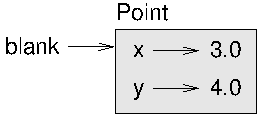
\includegraphics[scale=0.8]{../source/figs/point.pdf}}
\caption{Object diagram.}
\label{fig.point}
\end{figure}

The variable {\tt blank} refers to a Point object, which
contains two attributes.  Each attribute refers to a
floating-point number.

You can read the value of an attribute using the same syntax:

\begin{verbatim}
>>> blank.y
4.0
>>> x = blank.x
>>> x
3.0
\end{verbatim}
%
The expression {\tt blank.x} means, ``Go to the object {\tt blank}
refers to and get the value of {\tt x}.''  In the example, we assign that
value to a variable named {\tt x}.  There is no conflict between
the variable {\tt x} and the attribute {\tt x}.

You can use dot notation as part of any expression.  For example:

\begin{verbatim}
>>> '(%g, %g)' % (blank.x, blank.y)
'(3.0, 4.0)'
>>> distance = math.sqrt(blank.x**2 + blank.y**2)
>>> distance
5.0
\end{verbatim}
%
You can pass an instance as an argument in the usual way.
For example:
\index{instance!as argument}

\begin{verbatim}
def print_point(p):
    print('(%g, %g)' % (p.x, p.y))
\end{verbatim}
%
\verb"print_point" takes a point as an argument and displays it in
mathematical notation.  To invoke it, you can pass {\tt blank} as
an argument:

\begin{verbatim}
>>> print_point(blank)
(3.0, 4.0)
\end{verbatim}
%
Inside the function, {\tt p} is an alias for {\tt blank}, so if
the function modifies {\tt p}, {\tt blank} changes.
\index{aliasing}

As an exercise, write a function called \verb"distance_between_points"
that takes two Points as arguments and returns the distance between
them.


\section{Rectangles}
\label{rectangles}

Sometimes it is obvious what the attributes of an object should be,
but other times you have to make decisions.  For example, imagine you
are designing a class to represent rectangles.  What attributes would
you use to specify the location and size of a rectangle?  You can
ignore angle; to keep things simple, assume that the rectangle is
either vertical or horizontal.
\index{representation}

There are at least two possibilities:

\begin{itemize}

\item You could specify one corner of the rectangle
(or the center), the width, and the height.

\item You could specify two opposing corners.

\end{itemize}

At this point it is hard to say whether either is better than
the other, so we'll implement the first one, just as an example.
\index{Rectangle class}
\index{class!Rectangle}

Here is the class definition:

\begin{verbatim}
class Rectangle:
    """Represents a rectangle.

    attributes: width, height, corner.
    """
\end{verbatim}
%
The docstring lists the attributes:  {\tt width} and
{\tt height} are numbers; {\tt corner} is a Point object that
specifies the lower-left corner.

To represent a rectangle, you have to instantiate a Rectangle
object and assign values to the attributes:

\begin{verbatim}
box = Rectangle()
box.width = 100.0
box.height = 200.0
box.corner = Point()
box.corner.x = 0.0
box.corner.y = 0.0
\end{verbatim}
%
The expression {\tt box.corner.x} means,
``Go to the object {\tt box} refers to and select the attribute named
{\tt corner}; then go to that object and select the attribute named
{\tt x}.''

\begin{figure}
\centerline
{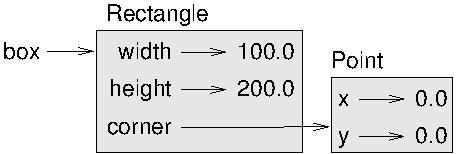
\includegraphics[scale=0.8]{../source/figs/rectangle.pdf}}
\caption{Object diagram.}
\label{fig.rectangle}
\end{figure}


Figure~\ref{fig.rectangle} shows the state of this object.
An object that is an attribute of another object is {\bf embedded}.
\index{state diagram}
\index{diagram!state}
\index{object diagram}
\index{diagram!object}
\index{embedded object}
\index{object!embedded}


\section{Instances as return values}
\index{instance!as return value}
\index{return value}

Functions can return instances.  For example, \verb"find_center"
takes a {\tt Rectangle} as an argument and returns a {\tt Point}
that contains the coordinates of the center of the {\tt Rectangle}:

\begin{verbatim}
def find_center(rect):
    p = Point()
    p.x = rect.corner.x + rect.width/2
    p.y = rect.corner.y + rect.height/2
    return p
\end{verbatim}
%
Here is an example that passes {\tt box} as an argument and assigns
the resulting Point to {\tt center}:

\begin{verbatim}
>>> center = find_center(box)
>>> print_point(center)
(50, 100)
\end{verbatim}
%

\section{Objects are mutable}
\index{object!mutable}
\index{mutability}

You can change the state of an object by making an assignment to one of
its attributes.  For example, to change the size of a rectangle
without changing its position, you can modify the values of {\tt
width} and {\tt height}:

\begin{verbatim}
box.width = box.width + 50
box.height = box.height + 100
\end{verbatim}
%
You can also write functions that modify objects.  For example,
\verb"grow_rectangle" takes a Rectangle object and two numbers,
{\tt dwidth} and {\tt dheight}, and adds the numbers to the
width and height of the rectangle:

\begin{verbatim}
def grow_rectangle(rect, dwidth, dheight):
    rect.width += dwidth
    rect.height += dheight
\end{verbatim}
%
Here is an example that demonstrates the effect:

\begin{verbatim}
>>> box.width, box.height
(150.0, 300.0)
>>> grow_rectangle(box, 50, 100)
>>> box.width, box.height
(200.0, 400.0)
\end{verbatim}
%
Inside the function, {\tt rect} is an
alias for {\tt box}, so when the function modifies {\tt rect},
{\tt box} changes.

As an exercise, write a function named \verb"move_rectangle" that takes
a Rectangle and two numbers named {\tt dx} and {\tt dy}.  It
should change the location of the rectangle by adding {\tt dx}
to the {\tt x} coordinate of {\tt corner} and adding {\tt dy}
to the {\tt y} coordinate of {\tt corner}.


\section{Copying}
\label{copying}
\index{aliasing}

Aliasing can make a program difficult to read because changes
in one place might have unexpected effects in another place.
It is hard to keep track of all the variables that might refer
to a given object.
\index{copying objects}
\index{object!copying}
\index{copy module}
\index{module!copy}

Copying an object is often an alternative to aliasing.
The {\tt copy} module contains a function called {\tt copy} that
can duplicate any object:

\begin{verbatim}
>>> p1 = Point()
>>> p1.x = 3.0
>>> p1.y = 4.0

>>> import copy
>>> p2 = copy.copy(p1)
\end{verbatim}
%
{\tt p1} and {\tt p2} contain the same data, but they are
not the same Point.

\begin{verbatim}
>>> print_point(p1)
(3, 4)
>>> print_point(p2)
(3, 4)
>>> p1 is p2
False
>>> p1 == p2
False
\end{verbatim}
%
The {\tt is} operator indicates that {\tt p1} and {\tt p2} are not the
same object, which is what we expected.  But you might have expected
{\tt ==} to yield {\tt True} because these points contain the same
data.  In that case, you will be disappointed to learn that for
instances, the default behavior of the {\tt ==} operator is the same
as the {\tt is} operator; it checks object identity, not object
equivalence.  That's because for programmer-defined types, Python doesn't
know what should be considered equivalent.  At least, not yet.
\index{is operator}
\index{operator!is}
\index{identity}
\index{equivalence}

If you use {\tt copy.copy} to duplicate a Rectangle, you will find
that it copies the Rectangle object but not the embedded Point.
\index{embedded object!copying}

\begin{verbatim}
>>> box2 = copy.copy(box)
>>> box2 is box
False
>>> box2.corner is box.corner
True
\end{verbatim}

\begin{figure}
\centerline
{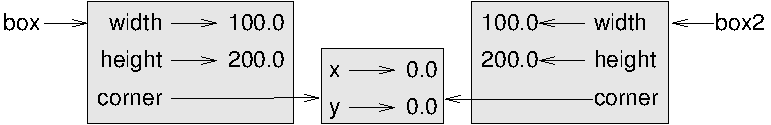
\includegraphics[scale=0.8]{../source/figs/rectangle2.pdf}}
\caption{Object diagram.}
\label{fig.rectangle2}
\end{figure}

Figure~\ref{fig.rectangle2} shows what the object diagram looks like.
\index{state diagram}
\index{diagram!state}
\index{object diagram}
\index{diagram!object}
This operation is called a {\bf shallow copy} because it copies the
object and any references it contains, but not the embedded objects.
\index{shallow copy}
\index{copy!shallow}

For most applications, this is not what you want.  In this example,
invoking \verb"grow_rectangle" on one of the Rectangles would not
affect the other, but invoking \verb"move_rectangle" on either would
affect both!  This behavior is confusing and error-prone.
\index{deep copy}
\index{copy!deep}

Fortunately, the {\tt copy} module provides a method named {\tt
deepcopy} that copies not only the object but also
the objects it refers to, and the objects {\em they} refer to,
and so on.
You will not be surprised to learn that this operation is
called a {\bf deep copy}.
\index{deepcopy function}
\index{function!deepcopy}

\begin{verbatim}
>>> box3 = copy.deepcopy(box)
>>> box3 is box
False
>>> box3.corner is box.corner
False
\end{verbatim}
%
{\tt box3} and {\tt box} are completely separate objects.

As an exercise, write a version of \verb"move_rectangle" that creates and
returns a new Rectangle instead of modifying the old one.


\section{Debugging}
\label{hasattr}
\index{debugging}

When you start working with objects, you are likely to encounter
some new exceptions.  If you try to access an attribute
that doesn't exist, you get an {\tt AttributeError}:
\index{exception!AttributeError}
\index{AttributeError}

\begin{verbatim}
>>> p = Point()
>>> p.x = 3
>>> p.y = 4
>>> p.z
AttributeError: Point instance has no attribute 'z'
\end{verbatim}
%
If you are not sure what type an object is, you can ask:
\index{type function}
\index{function!type}

\begin{verbatim}
>>> type(p)
<class '__main__.Point'>
\end{verbatim}
%
You can also use {\tt isinstance} to check whether an object
is an instance of a class:
\index{isinstance function}
\index{function!isinstance}

\begin{verbatim}
>>> isinstance(p, Point)
True
\end{verbatim}
%
If you are not sure whether an object has a particular attribute,
you can use the built-in function {\tt hasattr}:
\index{hasattr function}
\index{function!hasattr}

\begin{verbatim}
>>> hasattr(p, 'x')
True
>>> hasattr(p, 'z')
False
\end{verbatim}
%
The first argument can be any object; the second argument is a {\em
string} that contains the name of the attribute.
\index{attribute}

You can also use a {\tt try} statement to see if the object has the
attributes you need:
\index{try statement}
\index{statement!try}

\begin{verbatim}
try:
    x = p.x
except AttributeError:
    x = 0
\end{verbatim}

This approach can make it easier to write functions that work with
different types; more on that topic is
coming up in Section~\ref{polymorphism}.


\section{Glossary}

\begin{description}

\item[class:] A programmer-defined type.  A class definition creates a new
class object.
\index{class}
\index{programmer-defined type}
\index{type!programmer-defined}

\item[class object:] An object that contains information about a
programmer-defined type.  The class object can be used to create instances
of the type.
\index{class object}
\index{object!class}

\item[instance:] An object that belongs to a class.
\index{instance}

\item[instantiate:] To create a new object.
\index{instantiate}

\item[attribute:] One of the named values associated with an object.
\index{attribute!instance}
\index{instance attribute}

\item[embedded object:] An object that is stored as an attribute
of another object.
\index{embedded object}
\index{object!embedded}

\item[shallow copy:] To copy the contents of an object, including
any references to embedded objects;
implemented by the {\tt copy} function in the {\tt copy} module.
\index{shallow copy}

\item[deep copy:] To copy the contents of an object as well as any
embedded objects, and any objects embedded in them, and so on;
implemented by the {\tt deepcopy} function in the {\tt copy} module.
\index{deep copy}

\item[object diagram:] A diagram that shows objects, their
attributes, and the values of the attributes.
\index{object diagram}
\index{diagram!object}

\end{description}


\section{Exercises}

\begin{exercise}

Write a definition for a class named {\tt Circle} with attributes
{\tt center} and {\tt radius}, where {\tt center} is a Point object
and radius is a number.

Instantiate a Circle object that represents a circle with its center
at $(150, 100)$ and radius 75.

Write a function named \verb"point_in_circle" that takes a Circle and
a Point and returns True if the Point lies in or on the boundary of
the circle.

Write a function named \verb"rect_in_circle" that takes a Circle and a
Rectangle and returns True if the Rectangle lies entirely in or on the boundary
of the circle.

Write a function named \verb"rect_circle_overlap" that takes a Circle
and a Rectangle and returns True if any of the corners of the Rectangle fall
inside the circle.  Or as a more challenging version, return True if
any part of the Rectangle falls inside the circle.

Solution: \url{http://thinkpython2.com/code/Circle.py}.

\end{exercise}


\begin{exercise}

Write a function called \verb"draw_rect" that takes a Turtle object
and a Rectangle and uses the Turtle to draw the Rectangle.  See
Chapter~\ref{turtlechap} for examples using Turtle objects.

Write a function called \verb"draw_circle" that takes a Turtle and
a Circle and draws the Circle.

Solution: \url{http://thinkpython2.com/code/draw.py}.

\end{exercise}